\documentclass[a4paper]{article}

%---- PREAMBLE ----%

% Allows separate files to be used in the main file
\usepackage{subfiles}

% Algorithms
\usepackage{algorithm}
\usepackage[noend]{algpseudocode}
\renewcommand{\algorithmicrequire}{\textbf{Input:}}
\renewcommand{\algorithmicensure}{\textbf{Output:}}
\newcommand{\algorithmicbreak}{\State \textbf{break}}
\newcommand{\Break}{\algorithmicbreak}
\renewcommand{\algorithmicreturn}{\State \textbf{return}}
\newcommand{\algorithmicto}{\textbf{ to }}
\newcommand{\To}{\algorithmicto}
\newcommand{\algorithmicrun}{\State \textbf{call }}
\newcommand{\Run}{\algorithmicrun}
\newcommand{\algorithmicoutput}{\textbf{output }}
\newcommand{\Output}{\algorithmicoutput}
\newcommand{\algorithmictrue}{\textbf{true}}
\newcommand{\True}{\algorithmictrue}
\newcommand{\algorithmicfalse}{\textbf{false}}
\newcommand{\False}{\algorithmicfalse}
\newcommand{\algorithmicand}{\textbf{ and }}
\newcommand{\AAnd}{\algorithmicand}
\newcommand{\algorithmicnot}{\textbf{not}}
\newcommand{\Not}{\algorithmicnot}
\newcommand{\algorithmicor}{\textbf{ or }}
\newcommand{\Or}{\algorithmicor}

% Contains advanced math extensions
\usepackage{amsmath}

% Introduces the *proof* environment and the \theoremstyle command
\usepackage{amsthm}

% Adds new symbols to be used in math mode, e.g. \mathbb
\usepackage{amssymb}

% To declare multiple authors
%\usepackage{authblk}

% Provides extra comands as well as optimisation for producing tables
\usepackage{booktabs}
\newcommand{\ra}[1]{\renewcommand{\arraystretch}{#1}}

% Allows customisation of appearance and placements for figures/tables etc.
\usepackage{caption}

\usepackage{comment}

% Adds support for arbitrarily-deep nested lists
\usepackage[inline]{enumitem}

%Support for changing size of font in table footnotes
%\usepackage{etoolbox}

% Improves the interface for defining floating objects such as figures/tables
\usepackage{float}

%\usepackage{fullpage}

% For easy management of document margins and the document page size
\usepackage[a4paper]{geometry}

% Allows insertion of graphic files within a document
\usepackage{graphicx}

% Manage links within the document or to any URL when you compile in PDF
\usepackage[colorlinks]{hyperref} 
\usepackage[dvipsnames]{xcolor}
%Tikz colours, used in tikz figures only
\colorlet{tBlue}{RoyalBlue!35!Cerulean} %tikz color
\colorlet{tRed}{Red} %tikz color
\definecolor{tGreen}{HTML}{569909} %tikz color
\definecolor{tOrange}{HTML}{FA7602} %tikz color
\definecolor{tLightGreen1}{HTML}{C1E685} %tikz color
\definecolor{tLightOrange1}{HTML}{FFCD4F} %tikz color
\colorlet{tLightGreen}{LimeGreen!70!OliveGreen!45!White}
\colorlet{tLightOrange}{Dandelion!65!White}
\definecolor{tLightPink}{HTML}{FFD4EB} %tikz color
\definecolor{tLightBlue}{HTML}{CEF0FF} %tikz color

%Text colours
\colorlet{myRed}{Red!50!OrangeRed}
\definecolor{myOrange}{HTML}{FA7602}
\definecolor{myGreen}{HTML}{569909}
\definecolor{myAqua}{HTML}{00B1BA} %02BEB8
\definecolor{myBlue}{HTML}{0095FF} %00B3FF
\colorlet{myPurple}{Orchid} 
\colorlet{myPink}{Rhodamine!65!Lavender}
\colorlet{myGray}{Gray!90!White}

\hypersetup{
		linkcolor=myPurple,
		citecolor=myAqua,
		urlcolor=black
}

% The document class `elsarticle` uses the \AtBeginDocument comman to define the colour of all link types as blue, so we use the \AtBeginDocument command again to overwrite the colour settings to the colors we choose. REMEMBER TO REMOVE THIS BEFORE SUBMITTING.
%\AtBeginDocument{% 
%	\hypersetup{
%		linkcolor=myPurple,
%		citecolor=myAqua,
%		urlcolor=black
%	}
%} %end of \AtBeginDocument

\newcommand{\intro}[1]{{\color{myOrange}#1}} % \intro{<text>}, makes <text> orange, use to highlight things to do, urgent, or revisit in introduction section

\newcommand{\ahc}[1]{{\color{myBlue}#1}} % \ahc{<text>}, makes <text> blue, use to highlight things to do, urgent, or revisit in AHC section

\newcommand{\heur}[1]{{\color{myPink}#1}} % \scspp{<text>}, makes <text> pink, use to highlight things to do, urgent, or revisit in SCSPP section

\newcommand{\ea}[1]{{\color{myRed}#1}} % \ea{<text>}, makes <text> red, use to highlight things to do, urgent, or revisit in EA section

\newcommand{\cmsa}[1]{{\color{myGreen}#1}} % \cmsa{<text>}, makes <text> green, use to highlight things to do, urgent, or revisit in CMSA section

\newcommand{\conc}[1]{{\color{myPurple}#1}} % \conc{<text>}, makes <text> purple, use to highlight things to do, urgent, or revisit in Conclusion section

\newcommand{\note}[1]{{\color{myPurple}#1}} % \note{<text>}, makes <text> turquoise, use to highlight things to do, urgent, or revisit in any section


\newcommand{\alert}[1]{{\color{myRed}#1}} % \alert{<text>}, makes <text> red, use to highlight things to do, urgent, or revisit.

\newcommand{\done}[1]{{\color{myGray}#1}} % \done{<text>}, makes <text> gray, use to highlight things that are not required or should be ignored.

\newcommand{\ialert}[1]{{\color{myRed}\item#1}} % \ialert{<text>}, makes <text> a red bullet point, use for bullet points of things to do, urgent, or revisit.

\newcommand{\idone}[1]{{\color{myGray}\item#1}} % \idone{<text>}, makes <text> a gray bullet point, use for bullet points that have been completed, that are not required or should be ignored.

\renewcommand{\idone}[1]{} % hides all \idone bullet points

% Successor of amsmath
\usepackage{mathtools}

\usepackage{multirow}

% No indentation, space between paragraphs
%\usepackage{parskip}

\usepackage[round]{natbib}

%Include standalone .tex files
\usepackage{standalone}

% Define multiple floats (figures/tables) within one environment with individual captions 1a, 1b etc
\usepackage{subcaption}

%\usepackage[caption=false,font=footnotesize]{subfig}

\usepackage{tabularx}

\usepackage{threeparttable}
%\appto\TPTnoteSettings{\footnotesize} % Change font size of table footnotes to footnotesize

\usepackage{tikz}
\usetikzlibrary{shapes.geometric}

\usepackage{wrapfig}

% Need \usepackage{mathtools} to use floor/ceil below.
% Example: \floor*{\frac{x}{2}}, \ceil*{\frac{x}{2}}
% The asterisk resizes floor/ceil brackets.
\DeclarePairedDelimiter{\floor}{\lfloor}{\rfloor}
\DeclarePairedDelimiter{\ceil}{\lceil}{\rceil}

%Theorem style
%\theoremstyle{plain}% default
\newtheorem{theorem}{Theorem}
%\newtheorem{corollary}{Corollary}
\newtheorem{definition}{Definition}

%\theoremstyle{definition}
%\newtheorem{definition}{Definition}
%\newtheorem{proposition}{Proposition}
%\newtheorem{exmp}{Example}[section]
\usepackage{parskip}

\begin{document}
\title{\vspace{-20mm}Documentation: Abicare DST\vspace{-15mm}}
%\author{Asyl L. Hawa}
\date{}
\maketitle

\section{About the Program}
\begin{itemize}[leftmargin=*]
	\item Takes in an input file containing details for carers and clients availabilities and locations, and uses the information to produce a schedule and route for each carer to visit the clients.
	\item The algorithm used to determine a solution is a Greedy Randomised Adaptive Search Procedure (GRASP) combined with a Variable Neighbourhood Search (VNS) method, which is implemented in C. The pre- and post-processing of information is implemented in Python.
	\item This program is designed for use in social care to improve schedules/routes of carers to clients.
\end{itemize}

\section{Requirements}
\subsection{Code-Point Open}
The program uses Code-Point Open to obtain location data for carers and clients. Code-Point Open is available to download for free at https://www.ordnancesurvey.co.uk/business-government/products/code-point-open. The data format to download should be a CSV. Once the download is complete, extract the zip file and save the resulting \texttt{codepo\_gb} folder into the same directory as the program file.
\begin{itemize}[leftmargin=*]
	\item Code-Point Open is used to obtain exact locations from postcodes in the form of coordinates (latitude and longitude) from a free database provided by Ordnance Survey.
	\item Code-Point Open is a necessary requirement for the execution of the program.
\end{itemize}

\subsection{OSRM}
\begin{itemize}[leftmargin=*]
	\item The Open Source Routing Machine (OSRM) is an open-source router designed for use with data from the OpenStreetMap project.
	\item OSRM is used to obtain distances and travel times between coordinates.
	\item OSRM is a necessary requirement for the execution of the program.
\end{itemize}

\section{User Input Variables}
When the program is executed, a prompt will appear in which user input values can be provided for a number of parameters:
\begin{itemize}[leftmargin=*]
	\item Area name: the full name of the area to be scheduled and routed (default: Hampshire)
	\item Time window interval: the number of minutes before and after the expected start time of a job in which a carer can arrive and start the job (default: 15)
	\item Workload balance: a coefficient used to balance the workload for each carer (default: 1)
	\item Quality measure: the measure used to calculate the objective value (default: `Default')
	\item Time limit: the desired length of time (in seconds) for the algorithm to run (default: 60)
	\item Create website: the creation of an html website which displays the solution on a map (default: `Yes')
	\item Create plots: the creation of two plots showing the time information as a whole and the workload distribution for each carer (default: `Yes')
	\item Select file: the input file containing the carer and client details (.xlsx)
\end{itemize}

\begin{figure}[H]
	\centering
	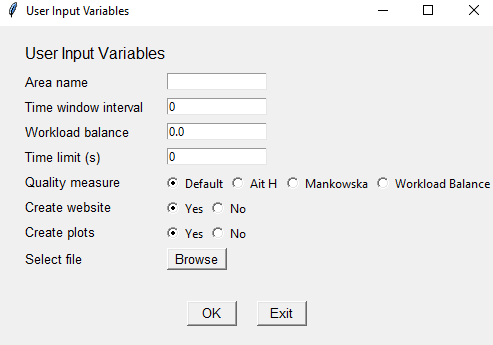
\includegraphics[width=0.6\linewidth]{figures/userinputscreenshot}%
\end{figure}

\section{Quality Measure Objective Functions}
The four quality measures, `Default', `Ait H', `Mankowska', and `Workload Balance', have different objective functions, calculated as follows:
\subsection{Default}
\begin{equation}
	\begin{split}
		\text{quality} &= (-1\times \text{total travel time}) + (-1 \times \text{total waiting time}) \\
		&+ (-5 \times \text{allowed tardiness}) + (-5 \times \text{total overtime}) \\
		&+ (\text{wb coefficient} \times \text{min spare time}) + \text{total preference score}
	\end{split}
\end{equation}
\noindent where the variable `wb coefficient' is the Workload Balance value provided by the user.

\subsection{Ait Haddadene}
\begin{equation}
	\text{quality} = -1\times ((0.3 \times \text{total travel time}) + \text{total preference score}) \\
\end{equation}

\subsection{Mankowska}
\begin{equation}
	\text{quality} = -1\times \frac{\text{total travel time} + \text{allowed tardiness} + \text{max tardiness}}{3} \\
\end{equation}

\subsection{Workload Balance}
\begin{equation}
	\begin{split}
		\text{quality} &= -1 \times ((0.3 \times \text{total travel time}) + \text{total preference score}) \\
		& + (-0.1 \times \text{length of day}) + (0.1 \times \text{min spare time})
	\end{split}
\end{equation}
\noindent where the variable `length of day' is the difference between the longest and shortest days in the solution.

\section{Output Files}
The program produces five output files: a text file, a CSV file, two image files containing plots, and a web file.
\subsection{Results File}
The results file is a text file (.txt) named as \texttt{area\_date\_results.txt}, where the area and date correspond to the area provided in the user input and the date for the schedule respectively.

The results file contains the following information:
\begin{enumerate}
	\item Date: the current date and time
	\item Quality: the final quality of the schedule and route produced by the program
	\item Measure: the quality measure used to calculate the quality of the solution
	\item Carers: the number of carers in the schedule
	\item Jobs: the number of jobs in the schedule
	\item Total time: the total amount of time for all carers in the schedule, including service time, travel time (excluding travel to and from carers' homes), waiting time, and overtime
	\item Total service time: the total amount of time for all jobs
	\item Total travel time: the total amount of time spent travelling for all carers (excluding travel to and from carers' homes)
	\item Total waiting time: the total amount of waiting time for all carers
	\item Total tardiness: the total amount of tardiness for all jobs
	\item Total overtime: the total amount of overtime for all carers
	\item Total mileage: the total distance travelled by all carers (excluding travel to and from carers' homes)
	\item Total cost: the total cost incurred by all carers as a combination of travel costs and mileage costs (excluding travel to and from carers' homes)
	\item Elapsed time: the total running time of the program
\end{enumerate}


\subsection{Solution File}
The solution file is a CSV file (.csv) named as \texttt{area\_date\_solution.csv}, where the area and date correspond to the area provided in the user input and the date for the schedule respectively.

The solution file contains the initial information provided for the clients, along with the following information for each job:
\begin{enumerate}
	\item carer\_id: the carer that is assigned to the job
	\item arrive\_job: the time at which the carer arrives at the job location
	\item start\_job: the time at which the carer starts the job
	\item depart\_job: the time at which the carer leaves the job location
	\item travel\_time: the time taken for the carer to travel to the job location from the previous job location (no travel time is provided for travel to the first job in a carer's route)
	\item waiting\_time: the amount of time between the arrival of the carer at the job location and the start of the job
	\item tardiness: the amount of time between the end of the job's time window and the start of the job 
\end{enumerate}

\subsection{Image Files}
There are two image files (.png) containing plots produced by the program. The files are named \texttt{area\_date\_time\_info.png} and \texttt{area\_date\_workload.png}, where the area and date correspond to the area provided in the user input and the date for the schedule respectively.

The \texttt{area\_date\_time\_info.png} file contains a pie chart depicting the percentage of total time spent on travel, waiting, and service.

The \texttt{area\_date\_workload.png} file provides a stacked bar chart depicting the time spent on travel, waiting, and service for each carer.

\subsection{Web File}
The final file produced is a web file (.html) which provides a visualisation of the schedule and route on a map. The file is named \texttt{area\_date.html}, where the area and date correspond to the area provided in the user input and the date for the schedule respectively.

\section{Possible Errors}
\begin{itemize}[leftmargin=*]
	\item If there is an incorrect postcode or missing postcode in the input file, an error will occur as the corresponding coordinates for the postcode will not be present in the Code-Point Open database.
	\item In this case, the postcode should be replaced with a neighbouring valid postcode.
\end{itemize}

\end{document}